
% An age profile with associated errors is available at the WAIS Divide ice core site (Buizert, personal communication 2016), however the  site lacks a robust measure of uncertainty. To derive Byrd ice core, we use volcanic events  detected in the Byrd ice core using the electrical conductivity method \citep{hammer1997}. We assume a 3\% uncertainty on the volcanic ages as a rule of thumb (personal communication, T.J. Fudge). We then invert for age given layer depth using a Bayesian MCMC approach and check our result by correlation to the nearby WAIS Divide ice core chronology.

% Our approach uses a Metropolis algorithm to fit an ice flow model to the observed volcanic profile from the Byrd ice core. An ensemble of well-fitting ice flow models is generated from this process which samples uncertainty in age given uncertainty in depth. We then sample from this ensemble to construct a distribution of likely ages for layers of interest. This method allows us to build a model using data from the last 50,000 years which can be used to estimate uncertainties in the chronology at earlier times.

To estimate the age-depth profile at the Byrd ice core, we use a Bayesian Markov Chain Monte Carlo technique to invert for the age and depth of observed englacial radar reflectors. This problem is nontrivial because the age of each reflector depends on solutions elsewhere in the ice column, so each is correlated with depth. As such, we choose an ensemble method because it would be inadequate to represent the age distribution as simply a standard deviation from mean values.

This method preserves the depth correlation of the ice chronology, estimates the probability of ice sheet parameter values, and develops a probabilistic estimate of the age-depth profile. A probabilistic approach is useful because while some parameters are well known, others are highly uncertain, such as the accumulation function at this site over time. By iteratively inverting for non-unique solutions, we find a distribution of sets of parameter values which are consistent with observations. Specifically, we derive an ensemble of age-depth profiles for the Byrd ice core constrained by agreement with a chronology of volcanic events from the past 50,000 years detected in the Byrd ice core record using the electrical conductivity method \citep{hammer1997}. 



\textbf{MOVE We assume a base level of 1\% uncertainty on the volcanic ages and include a precision parameter, \textit{S}, to quantify additional uncertainty. We invert for age given depth using a Bayesian Markov Chain Monte Carlo approach and check our result by correlation to the nearby WAIS Divide ice core chronology.}

The Bayesian formulation of this problem is:
\begin{equation}\label{bigproblem}
%\begin{split} %allow line break
%\begin{flalign}
%\begin{aligned}
p(A_r)  \sim \\ p(D_r, \vec{f},d_{firn},v_{ice},S | TWTT_r, A_{IC}, D_{IC})  \propto
p(TWTT_r | D_r,d_{firn},v_{ice} )~p(A_{IC}, D_{IC} | \vec{f},S)~p(D_r, f, S)~p(d_{firn})~p(v_{ice})\
%\end{flalign}
%\end{aligned}
%\end{split}
\end{equation}

Equation \ref{bigproblem} describes how we will estimate the depths of four englacial reflectors ($D_r$), ice flow model parameters ($\vec{f}$), firn depth correction ($d_{firn}), radar velocity in ice ($v_{ice}$), and a precision parameter on the uncertainty in the Byrd ice core chronology ($S$). Values for these quantities of interest will be informed by  information about observed reflector two-way travel time to each reflector observed by from radar ($TWTT_r$) and the age-depth profile from the Byrd ice core volcanic record ($A_{IC}$, $D_{IC}$). 

Priors on the quantities of interest as well as firn depth correction ($d_{firn}$) and velocity of electromagnetic waves in ice ($v_{ice}$), which contribute to errors in ice-penetrating radar depth, are used to put physical bounds on their values. Priors on ${D_r}$ also preserve stratigraphic dependence of radar reflectors, requiring deeper reflectors be older than shallower reflectors. The first two factors on the right-hand side of Equation~\ref{bigproblem} are likelihood functions. These describe the probability that modeled results agree with observations: in the first, agreement between observed two-way travel time ($TWTT_r$) and modeled reflector depths ($D_r$) and in the second, agreement between flow model results ($f$) and the volcanic ages ($A_{IC}$). 

The Metropolis algorithm is used to invert for parameter values consistent with observed ice core chronology and radar reflector data, effectively optimizing the likelihoods. Sets of parameter values for $D_r$, $\vec{f}$, $S$, $d_{firn}$, and $v_{ice}$ are proposed which sample uncertainty in age and depth. %This method allows us to build a model using data from the last 50,000 years which can be used to estimate uncertainties in the chronology at earlier times.
Likelihood functions for age, $p(A_{IC} | D_{IC},\vec{f},S)$, and TWTT, $p(TWTT_r | D_r,d_{firn},v_{ice})$, are evaluated to accept or reject proposed parameter sets based on how well they agree with the data. Accepted parameter values are those which are consistent with physical limits defined by the priors and with observations to within uncertainty. The resulting posterior probability distribution, $p(D_r, \vec{f},S | TWTT_r, A_{IC}, D_{IC})$, can then be used to deterministically compute the corresponding probability distribution of the age of observed radar reflectors, $p(A_r)$, using the flow model described below.


\subsubsection{Ice flow model at the Byrd ice core}
%This is consistent with experiment opinion that ice core age uncertainty is generally 2-3$\%$ of ice age (T.J. Fudge, private communication). Therefore, we construct an age-depth distribution for the Byrd ice core using statistical methods and an assumed 3$\%$ age uncertainty. The derived age-depth profile is then compared to the WAIS Divide profile using englacial layers that have been tracked between the two ice core sites. 

Due to the inherent stratigraphic dependence of age in the ice column, we use a flow model to simulate the age-depth relationship. We use a simple, one-dimensional model of ice flow (Equation \ref{schwander}) which derives ice age from accumulation and strain rate, assuming constant horizontal strain rate in the upper part of the ice sheet and a shear layer of thickness $h$ at the bottom of the ice sheet, for which we invert \citep{schwander2001}. In the shear layer, the strain rate is assumed to decrease linearly and the bottom of the ice is assumed sliding with velocity $q$ $\cdot$ $v_0$, where $v_0$ is the horizontal velocity at the surface.

\begin{equation}\label{schwander}
A(z) = \int_{z}^{H} \frac{dz}{\epsilon_z \dot{a}(z)}
\end{equation}
where
\begin{center}
$    \epsilon_z=
    \begin{cases}
                 1-k(H-z), & h \leq z \leq H \\
                  kz(q+\frac{1-q}{2h}z), & 0 < z < h
    \end{cases}, 
$
$
k = \frac{2}{2H - h(1-q)}
$
\end{center}
$H$ is ice thickness in ice equivalent, $z$ is height above the bed, $h$ is the depth to the shear layer, $\dot{a}$ is the layer thickness, and $q$ is a constant for which we invert. 

The ice flow model accounts for two primary factors in the age-depth profile: burial as a function of accumulation rate, $\dot{a}$, and thinning as a function of strain, $\epsilon_z$. In the simplest realization, ice deposited at a given time at the ice sheet surface will be found at a depth in the ice sheet corresponding to the amount of subsequent accumulation. However, due to strain thinning at depth, the ice will be less deep than would be expected if accumulation alone is considered. 

In Section~\ref{metrop}, we invert for the flow parameters $h$, $q$, and $\dot{a}$. Constant values for $h$ and $q$ are sampled from uniform priors defined in a conservative range. Accumulation is estimated for 11 units of depth spaced every 200 m starting from the ice surface and are sampled from the same uniform prior.

\begin{center}
%\begin{equation}
$p(\vec{f}) = 
	\begin{cases}
		p(h) \sim U(0, 0.5) \\
		p(q) \sim U (0, 1) \\
		p(\dot{a}_{z < 200 m ... z > 2000 m}) \sim U(0.5~m/a,0.15~m/a)\\
	\end{cases}
$	
%\end{equation}	
\end{center}

The prior distributions of flow parameters, together denoted as $p(\vec{f})$, assume the shear layer is in the bottom half of the ice sheet depth and that the bed of the ice sheet is moving slower than the surface. Accumulation as a function of depth, $\dot{a}$, is sampled from 11 distinct depth bins spanning the ice thickness. This allows for variability of accumulation over time, as expected. To limit unrealistic variability in accumulation between depth bins, Tikhonov regularization is used on the age likelihood function to punish estimates of the accumulation function which are highly-variable relative to a solution computed with no regularization and smoothed over a moving 600-m depth window.




\subsection{Radar depth and error model}
 Radar pulses transmitted into the ice sheet reflect off surfaces of dielectric contrast in the ice that are the result of variations in ice fabric, composition, temperature, and rheology of ice \citep{fujita2000}. The reflected signal is received by the radar system and recorded as two-way travel time (TWTT) from transmission to receipt.  The reflector data in this analysis (Figure~\ref{fig:layergram}) were collected by the University of Texas Institute for Geophysics, including GIMBLE \citep{gimble2017}, AGASEA \citep{holt2006}, CASERTZ \citep{morse2002}, and SOAR/WMB \citep{luyendyk2003} (Figure~\ref{fig:radarmap}). Data used to trace reflectors between Byrd ice core and WAIS Divide ice core were collected from a DC-3 or Twin Otter airborne platform and used the HiCARS coherent radar system with 60 MHz center frequency and 15 MHz bandwidth \citep{peters2005}.% or the TUD-derived incoherent radar sounder \citep{blankenship2001} with 4 MHz bandwidth.

\begin{figure}[h]
\centering
\makebox[\textwidth][c]{
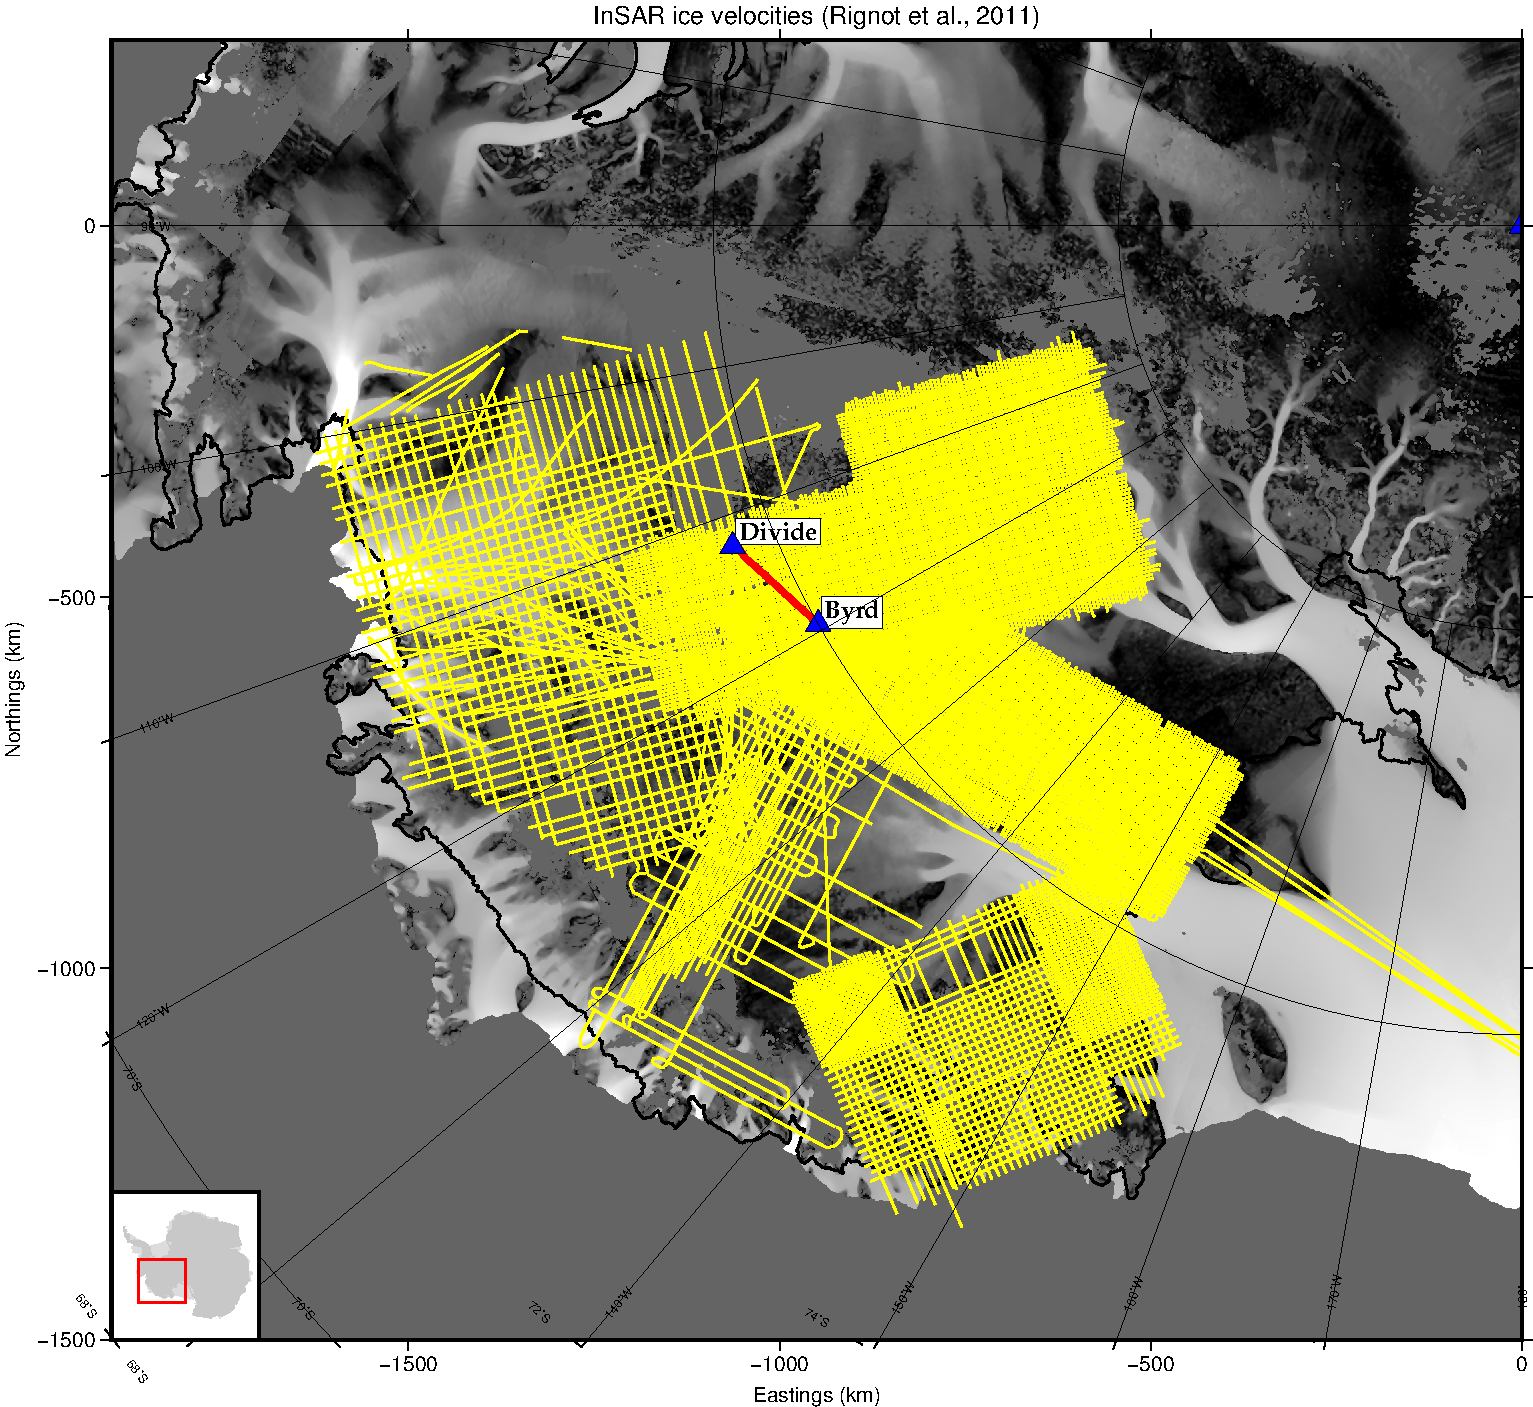
\includegraphics[scale=0.5]{/Users/gail/Documents/Research/Projects/Layers/analysis/figures/WAIS_vel_gray_final}}
%\captionsetup{width=.9\textwidth}
\caption{Map of central West Antarctic with available airborne geophysical radar surveys (yellow lines) and  WAIS Divide and Byrd ice core locations (blue triangles) overlain. Gray shading is surface velocity \citep{rignot2011}. The red line denotes the flight line along which the reflectors in this study were observed. }
\label{fig:radarmap}
\end{figure}



In this study, we consider TWTT of four reflectors spanning the ice thickness in the region of central West Antarctica (Figure~\ref{fig:layergram}). These reflectors have been tracked using Halliburton's Landmark seismic interpretation software and can be tied to both the Byrd and WAIS Divide ice cores for dating using observations from the HiCARS system (Figure~\ref{fig:radarmap}). %Determining the depth of the reflectors, $D_r$, may be affected by several sources of uncertainty, including uncertainty in the firn depth, the velocity of the radar pulse in ice, and the pulse-limited precision of radar observations.

\begin{figure}[h]
\centering
\makebox[\textwidth][c]{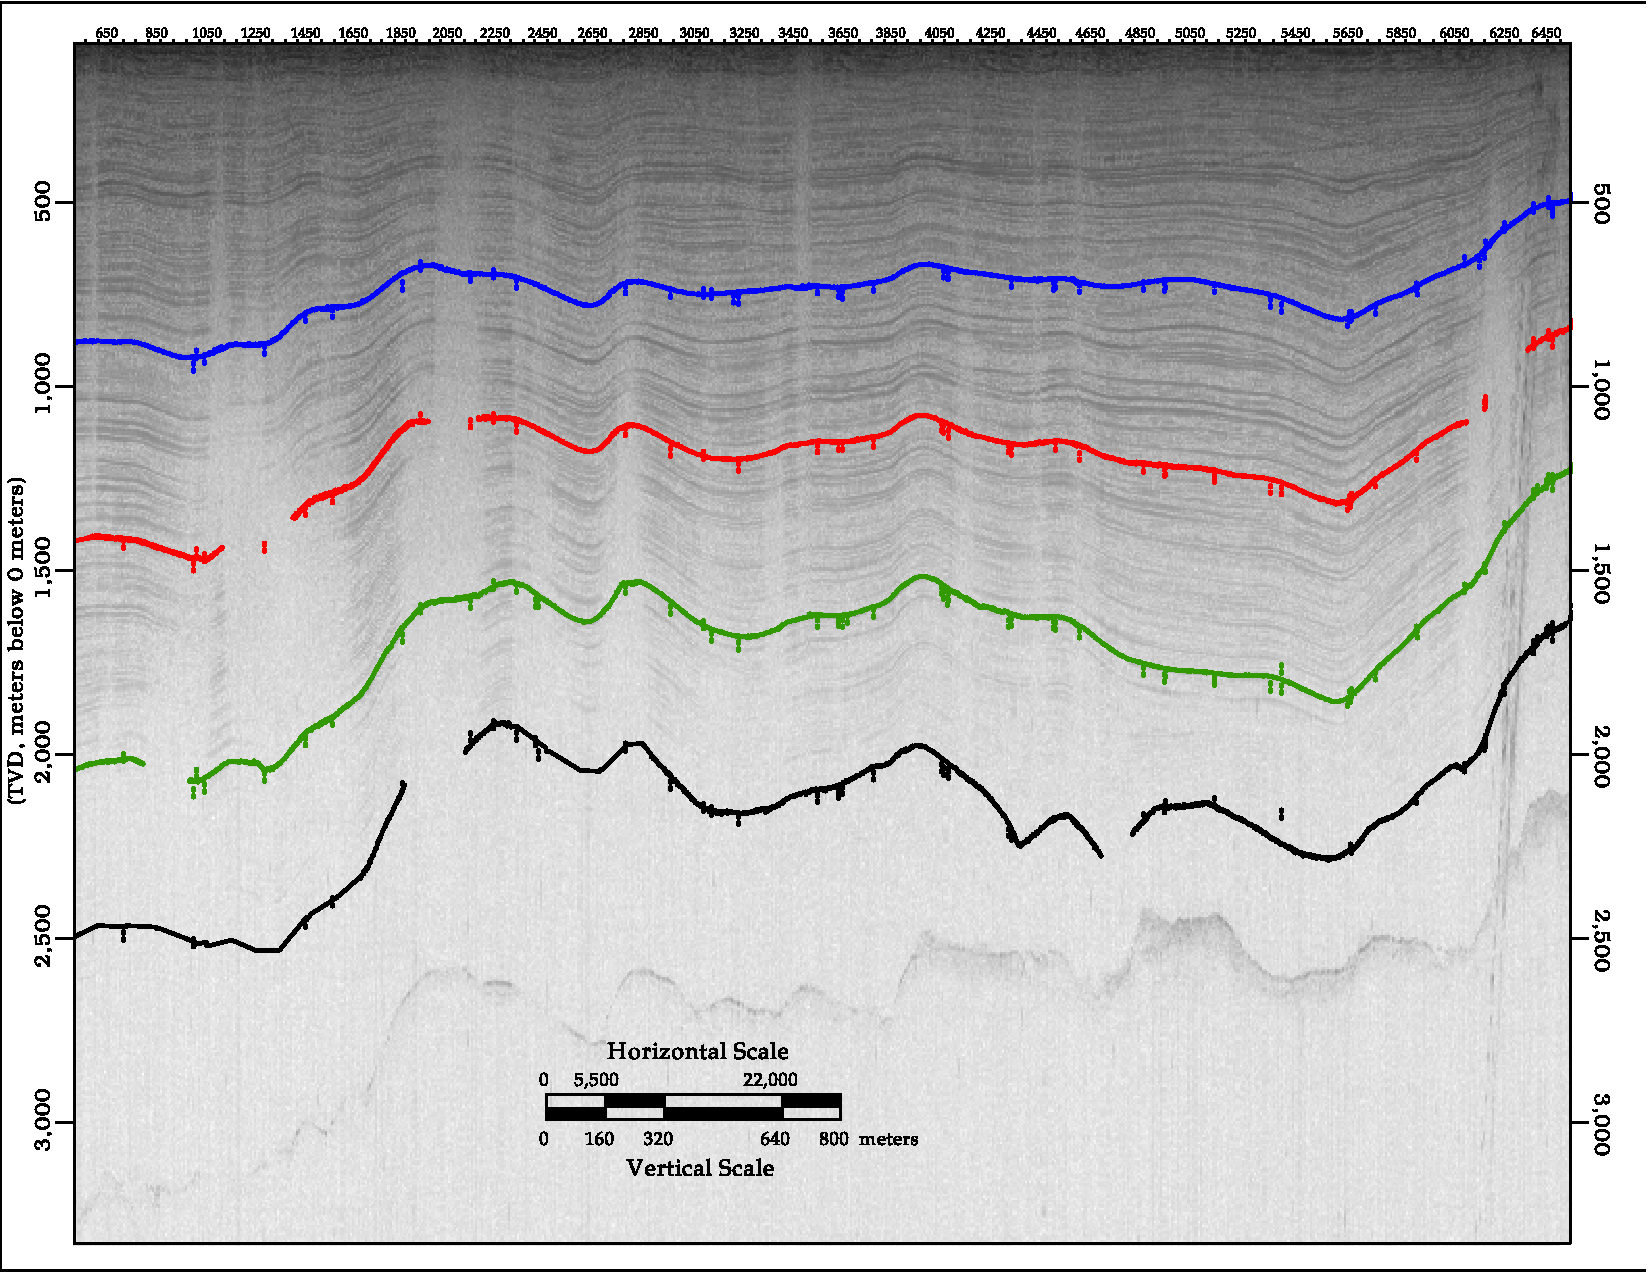
\includegraphics[scale=0.6]{/Users/gail/Documents/Research/Projects/Layers/paper/figures/radargram-4layers-paper}}
%\captionsetup{width=.9\textwidth}
\caption{Radargram showing reflectors of interest near the Byrd ice core along flight line ICP6/MKB2l/F14T01a observed using the HiCARS2 radar system. Short vertical hatches along tracked reflectors show intersections with crosslines.}
\label{fig:layergram}
\end{figure}


To estimate reflector depths from TWTT ($TWTT_{m,r}(D_r)$), we use a simple relation between the different velocities of the radar signal in air and in ice and incorporate several known sources of uncertainty, including: 1) variations in the radar velocity in ice due to ice temperature and fabric ($v_{ice}$), 2) vertical precision limitations of radar range detection ($\sigma_{prec}$), and 3) uncertainty in the firn correction ($\epsilon_{firn}$) due to measurement errors in the ice density profile:

\begin{equation}\label{deptheqn}
%D_r= \frac{1}{2}[(TWTT_r + \epsilon_{prec,r}) - (TWTT_{surf} + \epsilon_{prec,surf})] \cdot v_{ice} + d_{firn}\\
TWTT_{m,r}(D_r) + \sigma_{prec,r} = 2 \frac{D_r - (d_{firn}+\epsilon_{firn})}{v_{ice}} + (TWTT_{surf} + \epsilon_{prec,surf})
\end{equation}

The complexity of local ice properties affecting the velocity at any location and depth make it difficult to know the true velocity. Empirical evidence suggests a range of expected velocities and we conservatively assume they are uniformly distributed such that: $p(v_{ice}) ~\sim U[168,169.5]\,m/{\mu}s$ \citep{fujita2000}. In lieu of detailed observations of ice properties with depth, we assume the value of $v_{ice}$ is a constant throughout the ice column and apply it systematically to all reflector depths.

The radar pulse width determines vertical precision, $\sigma_{prec,r}$ \citep{millar1982}. We assume a finite pulse width, meaning an infinitesimally thin layer of ice will appear in the survey to have a finite width. This can lead to errors in tracing isochronous reflectors, as the reflected energy from a finite depth will include ice with a range of ages. To account for this, we include uncertainty due to range precision, according to the signal to noise ratio of each reflector's radar amplitude as in \citet{cavitte2016}:

\begin{equation}
\sigma_{prec,r} = \frac{\Delta{r}}{\sqrt{SNR_r}}
\end{equation} 
The range resolution, $\Delta{r}$, is 8.4 m for all reflectors in the HiCARS2 system \citep{young2011}. Values of the SNR for each reflector are shown in Table~\ref{tab:depthunc}. 

%We assume this error is normal such that $p(\epsilon_{prec}) = N(0,\sigma_r)$ ns. Values of $\epsilon_{prec}$ are sampled for each reflector independently.

Finally, a firn layer with variable density \citep{gow1970} exists in the upper part of the ice sheet. The velocity of the radar is faster in firn than in solid ice. To correct for the underestimation of ice depth if the firn layer is not considered, we estimate the firn correction ($d_{firn}$), the difference between the ice thickness with and without the firn layer present . %Based on the density profile and firn thickness ($\sim$ 65 m) at the Byrd ice core site \citep{gow1970}, we estimate the prior on $d_{firn}$ to be $p(d_{firn})\sim$ U[6, 36]\,m. This assumes firn density ranges from 400 - 8030 $\frac{kg}{m^3}$ and glacial ice ranges from 830 - 917 $\frac{kg}{m^3}$ \citep{paterson1994}. The firn correction is applied to all estimates of englacial reflector depth in this study because they are all deeper than the measured firn layer.
Errors in density, $\rho(z)$, are used to estimate the error in $d_{firn}$, $\epsilon_{firn}$. These errors are known for the WAIS Divide measurements, but not for the Byrd ice core profile. In lieu of density measurement errors at the Byrd site, we assume the errors to be consistent with those observed at the WAIS Divide ice core. These errors are assumed gaussian, randomly sampled, and the firn correction is computed using the \citet{dowdeswell2004} relation:

\begin{equation}
d_{firn} = \frac{K}{n^{'}_{i}}\int{(\rho_{i} - \rho(z)) dz}
\end{equation}
where K is 0.85 m$^{3}$ Mg$^{-1}$ \citep{robin1969}, $n^{'}_{i}$ is the refractive index of ice ($n^{'}_{i}$=1.78), $\rho_{i}$ is the density of ice ($\rho_{i}$=0.917 Mg m$^{-3}$) and $\rho(z)$ is the density of ice at depth \textit{z} with units Mg m$^{-3}$.

The TWTT from the observing aircraft to the surface of the ice sheet is known from interpretation of the surface reflector, $TWTT_{surf}$. The computed depth of each reflector is relative to this surface reflector. Just as each reflector may have TWTT precision errors independent of the others, errors in the distance between the surface and the acquisition aircraft are common to all observed reflectors in the ice column. Therefore, a randomly sampled precision error, $\epsilon_{prec,surf}$, is applied systematically to all reflectors.







\label{radardepth}
\subsection{Metropolis Algorithm}\label{metrop}
At each iteration, the Metropolis/Gibbs sampling algorithm \citep{metropolis1953,hastings1970} proposes values for parameters of interest (those with priors in Equation~\ref{eqn:bigproblem}). The algorithm accepts or rejects proposed sets of parameter values by comparison between the proposed and previously-accepted likelihood (or ``cost") values. A low cost value represents good agreement between model and observations, reflecting a small model-data misfit. According to the Metropolis/Gibbs algorithm, if the cost associated with proposed parameters is lower than that of the last accepted iteration, the proposed parameter values are accepted. Alternatively, higher cost values may be accepted with a probability determined by the likelihood. Each likelihood function is considered separately and both must represent an adequate solution on a given iteration for the proposed parameters to be accepted.


There are two likelihood functions, describing the model-data misfit between reflector depth and age, respectively:


\begin{equation}\label{eqn:loglikeage}
p(A_{IC} | D_{IC},\vec{f},S) \propto exp[\frac{-S\sum_{j = 61}[A_{IC,j} - A_{m,j}(\vec{f},D_{IC})]^2}{2\sigma_A^2} + r^6]
\end{equation}

\begin{equation}\label{eqn:loglikedepth}
p(TWTT_r | D_r,d_{firn},v_{ice} ) \propto exp[\frac{-\sum_{i=4}[TWTT_{r,i} - TWTT_{m,i}(D_r)]^2}{2\sigma_{TWTT}^2}]
\end{equation}


In the depth likelihood function, $TWTT_m(D_r)$ is based on the relationship between depth and TWTT as in Equation~\ref{deptheqn} and $TWTT_r$ is observed by ice-penetrating radar for each reflector, $i$. To estimate $\sigma_{TWTT}$, we assume a perfect model and compute with standard deviation of the numerator given typical errors we expect affect our data. This method allows for correlation between depth errors, as expected. More details are discussed in the Supplement.


In the age likelihood function, the modeled age, $A_m$, is a function of ice flow model parameters, $\vec{f}$. A regularization term, $r^6$, is used to penalize large variability in the sampled accumulation rate function input to the ice flow model and $A_m$ comes from solutions to the forward ice flow model. We train our model on $J=61$ volcanic events from \citet{hammer1997}. Importantly, these volcanic ages are overly confident in that they do not include uncertainty information. To accomodate additional unknown uncertainty in this data, we include an unknown precision parameter, $S$, and use it to infer uncertainty in the volcanic record from scatter between our model and the observed data. $S$ is a ``nuisance" parameter that accounts for uncertainty in $\sigma_A$ by using $E_m$ as a measure of scatter between modeled age $A_m$ and $\Pi(S) \propto Ga(\alpha,\beta)$ The posterior probability distribution of $S$ is therefore:

\begin{equation}\label{eqn:S}
PPD(S) = Ga(\frac{k_e}{2}+\alpha, E_m+\beta)
\end{equation}
where 
\begin{equation}
 E_m= \frac{\sum_{j}[A_{IC,j} - A_{m,j}(\vec{f},D_{IC})]^2}{2\sigma_A^2} 
\end{equation}

Parameters $\alpha$ and $\beta$ are assumed to be 1 as in the case for a noninformative gamma prior. The scatter between the model and data is represented by the cost, $E_m$, which determines the uncertainty. The number of degrees of freedom, $k_e$, is assumed to be less than $J$ due to covariation in the age and depth of ice. Because we do not know the value of $k_e$ a priori, we assume $k_e = \frac{J}{2}$ (see Supplement). Unlike other parameters in our problem in which Metropolis-Hastings sampling is used, values of $S$ are proposed using Gibbs sampling \citep{gelfand1992}, effectively estimating reflector age uncertainty given the choice of parameter solution for each iteration.


%The Metropolis algorithm randomly samples each of the ice flow parameters and computes an age-depth profile. A Bayesian method is used to determine suitability of proposed ice flow parameters in a Bayesian way:
%\begin{equation}\label{posterior}
% p(\vec{f},\sigma_V | A_V, D_V) \propto p(A_V,D_V | \vec{f},\sigma_V) p(\vec{f}) p(\sigma_V),
%\end{equation}
%A posterior probability, $p(A | \vec{f})$, is computed for each set of parameters from likelihood and prior probabilities, $P(\vec{f})$. As described below, we require only the proportional relation because relative posterior values are considered in this Markov Chain process.

%The simulated age-depth profile is compared to the observed volcanic chronology using the ``log-likelihood" function, $p(A_V,D_V | \vec{f},\sigma_V)$, to quantify how closely a sampled set of parameters represents the observed ice profile:
%
%\begin{equation}\label{cost}
%ln(likelihood) = \frac{1}{N}\sum\frac{(A_{sim}(\vec{f})_i~ - ~A_{V,i})^2}{(2\sigma_{V})^2},
%\end{equation}
%where $\vec{Age}_{sim}$ comes from evaluating the ice flow model for parameter values sampled from $\vec{f}$. $A_{V}$ and $\sigma_{V}$ describe the observed volcanic chronology at the Byrd ice core. The prior on $\sigma_{V}$ is 
%\begin{equation}
%p(\sigma_V) \sim Ga(\alpha, \beta)
%\end{equation}

%which assumes error in the chronology is $\sim$3\% (T.J. Fudge, pers. comm.). Uncertainty in the volcanic chronology, $\sigma_{V}$, loosens the constraint on how closely $A_{sim}$ must match $A_{V}$ to be acceptable. We assume $N$ degrees of freedom, where $N$ is the number of volcanic observations. This is because observed global volcanic events are assumed independent.
%



%\subsubsection{Estimating accumulation}\label{accum}
The accumulation rate, $\dot{a}$, is highly uncertain for the Byrd ice core, so we compare ice flow model solutions using several accumulation functions. These include constant accumulation, a theoretical function derived for an expected atmospheric temperature timeseries at the nearby WAIS Divide ice core\citet{morse2002}, constant accumulation rates every 5,000 years, and constant accumulation rates in four depth bins which correspond to observed changes in layer thickness at the byrd ice core \citep{}. \textbf{Adding an accumulation function based on Byrd ice core isotopes.}

The result is shown in Figure \ref{fig:accumfunc}. We see that \textbf{One of them does better than the others. This one will be used in the final model to give the real result of age-depth for all the reflectors.}


%\begin{figure}
%%\begin{center}
%\centering
%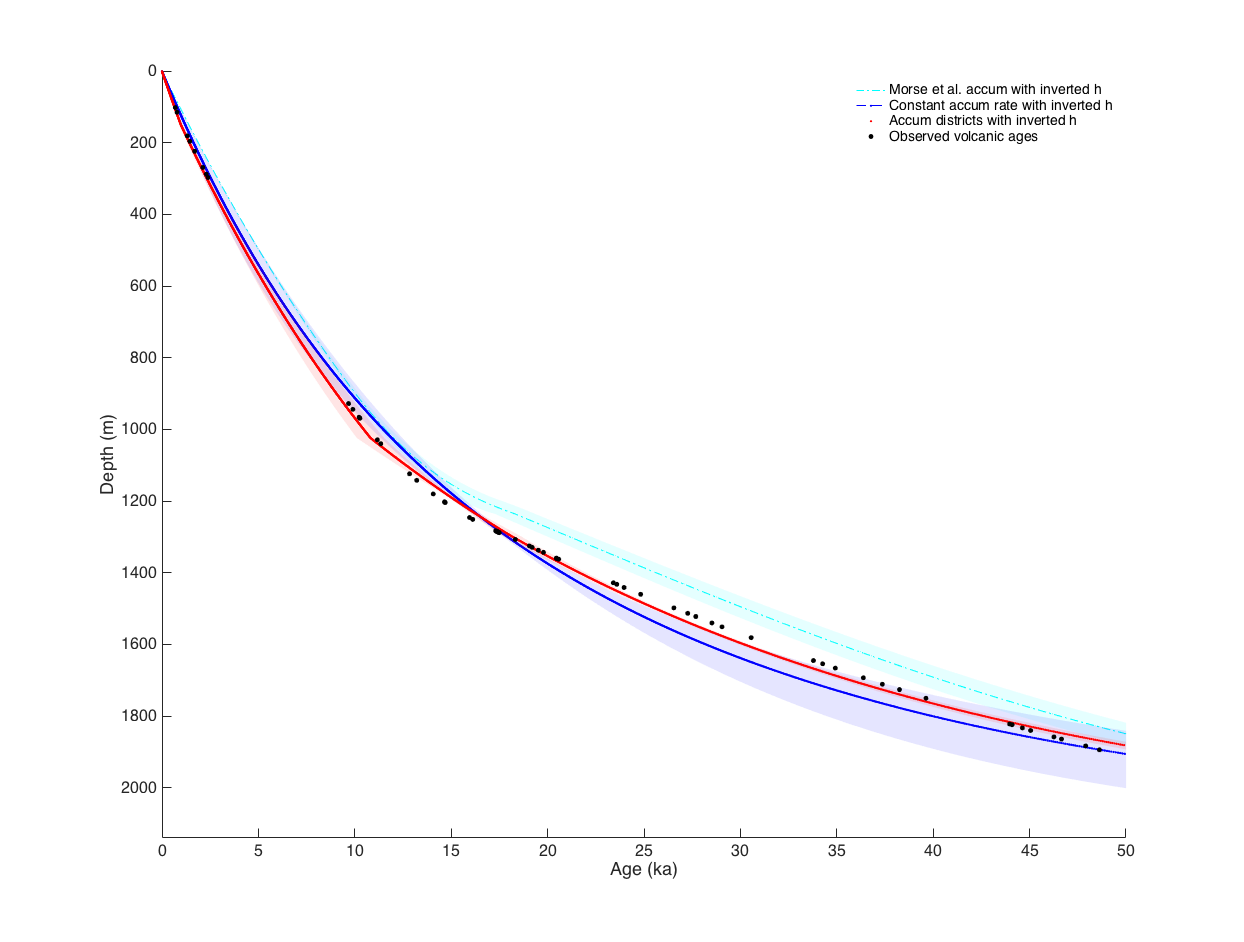
\includegraphics[scale=0.4]{figures/accumfunc}
%%\captionsetup{width=.9\textwidth}
%\caption[]{\textbf{Unfortunately, this figure is missing the 5k year interval which is the best (but takes the longest to run). In general, the accumulation functions fit the volcanic data well, but perhaps too well as seen in the comparison with the WAIS Divide ice core. This is a proof of concept that the data can be modeled using the MCMC method and we therefore can compute an age-depth profile even where there is no data, but the uncertainty so far is being underestimated.}}
%%\end{center}
%\label{fig:accumfunc}
%\end{figure}



